\documentclass[final]{article}
\usepackage[numbers,sort&compress]{natbib} % formato de citas
\usepackage{neurips}            % estilo de la conferencia NeurIPS
\usepackage[spanish]{babel}     % definiciones para el español
\usepackage{graphicx}           % para insertar figuras
\usepackage{amsmath,amssymb}    % más símbolos útiles
\usepackage[hidelinks]{hyperref}% para los links
\usepackage[ruled,vlined,lined,linesnumbered,spanish,onelanguage]{algorithm2e}
\usepackage{multirow}
\usepackage{booktabs}
\usepackage{float}

\begin{document}
\def\tablename{Tabla}          % (sino les pone Cuadro)

\title{Detección de Anomalías Industriales en Tornillos mediante
       Procesamiento Digital de Imágenes}

\author{A. Glorioso y A. Meier \\
        Facultad de Ingeniería y Ciencias Hídricas, \\
        Universidad Nacional del Litoral}

\maketitle

\begin{abstract}
La inspección visual automática de piezas industriales exige métodos rápidos,
interpretables y de bajo costo computacional. Este trabajo aborda la detección
de defectos de fabricación en tornillos utilizando exclusivamente técnicas
clásicas de procesamiento digital de imágenes, sin recurrir a redes neuronales,
aprovechando las condiciones controladas de la inspección industrial
(iluminación estática y fondo uniforme). Se propone un sistema basado en
detección de anomalías por modelo de referencia: a partir de imágenes de
tornillos sanos se construye una plantilla estadística del objeto, y toda
desviación respecto de ella se interpreta como un defecto potencial. El
pipeline normaliza la pose de cada pieza mediante segmentación por bordes y
alineación por momentos, y luego aplica tres detectores complementarios
(forma, intensidad y perfil de rosca) cuyos resultados se cuantifican por
región y se contrastan contra umbrales calibrados estadísticamente con la regla
de las tres sigmas. Evaluado sobre la categoría \emph{screw} del dataset
público MVTec AD (160 imágenes), el sistema alcanza un 95{,}6\% de exactitud
en la clasificación binaria normal/anómala con cero falsos positivos,
identificando además el tipo y la ubicación del defecto.
\end{abstract}

%==========================================================
\section{Introducción}

La detección automática de defectos superficiales y estructurales es un
problema central en el control de calidad industrial. En entornos de
inspección controlados —iluminación fija, fondo uniforme y objeto centrado—
es posible diseñar algoritmos basados en el análisis de la geometría, los
contornos y los cambios de intensidad, que resultan rápidos, altamente
interpretables y de bajo costo computacional frente a las soluciones basadas
en aprendizaje profundo.

El presente trabajo se enmarca en la tarea de \emph{detección de anomalías}
(\textit{anomaly detection}): a diferencia de un clasificador supervisado
clásico, no se dispone de un conjunto representativo de cada tipo de defecto,
sino fundamentalmente de ejemplos de piezas correctas. El dataset de referencia
en esta área es MVTec AD~\cite{bergmann2019mvtec}, diseñado específicamente
para evaluar métodos de detección de anomalías no supervisada en escenarios
industriales reales. Su categoría \emph{screw} es reconocida como una de las
más difíciles del conjunto, debido a la rotación arbitraria de la pieza y a la
sutileza de varios de los defectos.

Gran parte de la literatura reciente aborda MVTec AD mediante redes neuronales
profundas (autoencoders, modelos de \textit{embeddings} preentrenados o flujos
normalizados)~\cite{bergmann2019mvtec}. Estos métodos alcanzan alta exactitud
pero a costa de interpretabilidad y recursos. En contraste, las técnicas
clásicas de procesamiento de imágenes —umbralado de Otsu~\cite{otsu1979},
detección de bordes de Canny~\cite{canny1986} y morfología
matemática~\cite{gonzalez2018}— permiten construir sistemas cuyo razonamiento
es completamente trazable: cada decisión puede explicarse en términos de una
medida geométrica o de intensidad concreta. Esta característica resulta
especialmente valiosa en contextos industriales donde se requiere justificar
el rechazo de una pieza.

En consonancia con los objetivos de la asignatura, se propone un sistema que
detecta defectos en tornillos empleando \emph{únicamente} técnicas clásicas.
La contribución principal es el diseño de \textbf{tres detectores
complementarios} —de forma, de intensidad y de perfil de rosca— cada uno
dirigido a una familia de defectos identificada mediante un análisis previo
del dataset, integrados sobre una etapa de normalización de pose que hace
comparables todas las imágenes píxel a píxel.

%==========================================================
\section{Materiales y Métodos}

\subsection{Base de datos}

Se utilizó la categoría \emph{screw} del dataset MVTec
AD~\cite{bergmann2019mvtec}, compuesta por imágenes en escala de grises de
$1024\times1024$ píxeles, con el tornillo centrado sobre un fondo claro y
uniforme. Las 160 imágenes se distribuyen en seis grupos: 41 piezas sanas
(\emph{good}) y 119 con defectos repartidos en cuatro tipos:
arañazos en la cabeza (\emph{scratch\_head}, 24) y en el cuello
(\emph{scratch\_neck}, 25), roscas deformadas (\emph{thread\_side} 23 y
\emph{thread\_top} 23) y puntas manipuladas (\emph{manipulated\_front}, 24).
Las herramientas de desarrollo fueron Python con las librerías OpenCV, NumPy
y Matplotlib.

\subsection{Análisis del dataset y estrategia general}

Un análisis visual sistemático de las seis categorías permitió caracterizar
cada defecto y orientar el diseño (Tabla~\ref{tab:defectos}). Se observaron dos
familias bien diferenciadas: los \emph{arañazos} (cabeza y cuello) alteran la
\emph{intensidad} interna pero no el contorno de la pieza, mientras que las
\emph{roscas y puntas dañadas} alteran la \emph{silueta}. Esta dicotomía
descarta la existencia de un detector único y motiva el enfoque
multi-detector.

\begin{table}[h]
\centering
\caption{Caracterización de los defectos a partir del análisis del dataset.}
\label{tab:defectos}
\small
\begin{tabular}{lll}
\toprule
\textbf{Tipo} & \textbf{Región} & \textbf{Manifestación} \\
\midrule
scratch\_head      & cabeza & estrías brillantes (intensidad) \\
scratch\_neck      & cuello & raspones claros u oscuros (intensidad) \\
thread\_side/top   & rosca  & rebabas y muescas (silueta) \\
manipulated\_front & punta  & doblada o truncada (silueta) \\
\bottomrule
\end{tabular}
\end{table}

Se adoptó un esquema de \textbf{detección por modelo de referencia}: se
construye una plantilla estadística del tornillo sano a partir de las 41
imágenes \emph{good}, y toda desviación significativa respecto de ella se
interpreta como anomalía. El pipeline completo (Fig.~\ref{fig:pipeline})
consta de cinco fases agrupadas en dos etapas: \emph{normalización} de la pose
(segmentación y alineación) y \emph{comparación} contra la referencia
(detección, cuantificación y clasificación).

\begin{figure}[h]
\centering
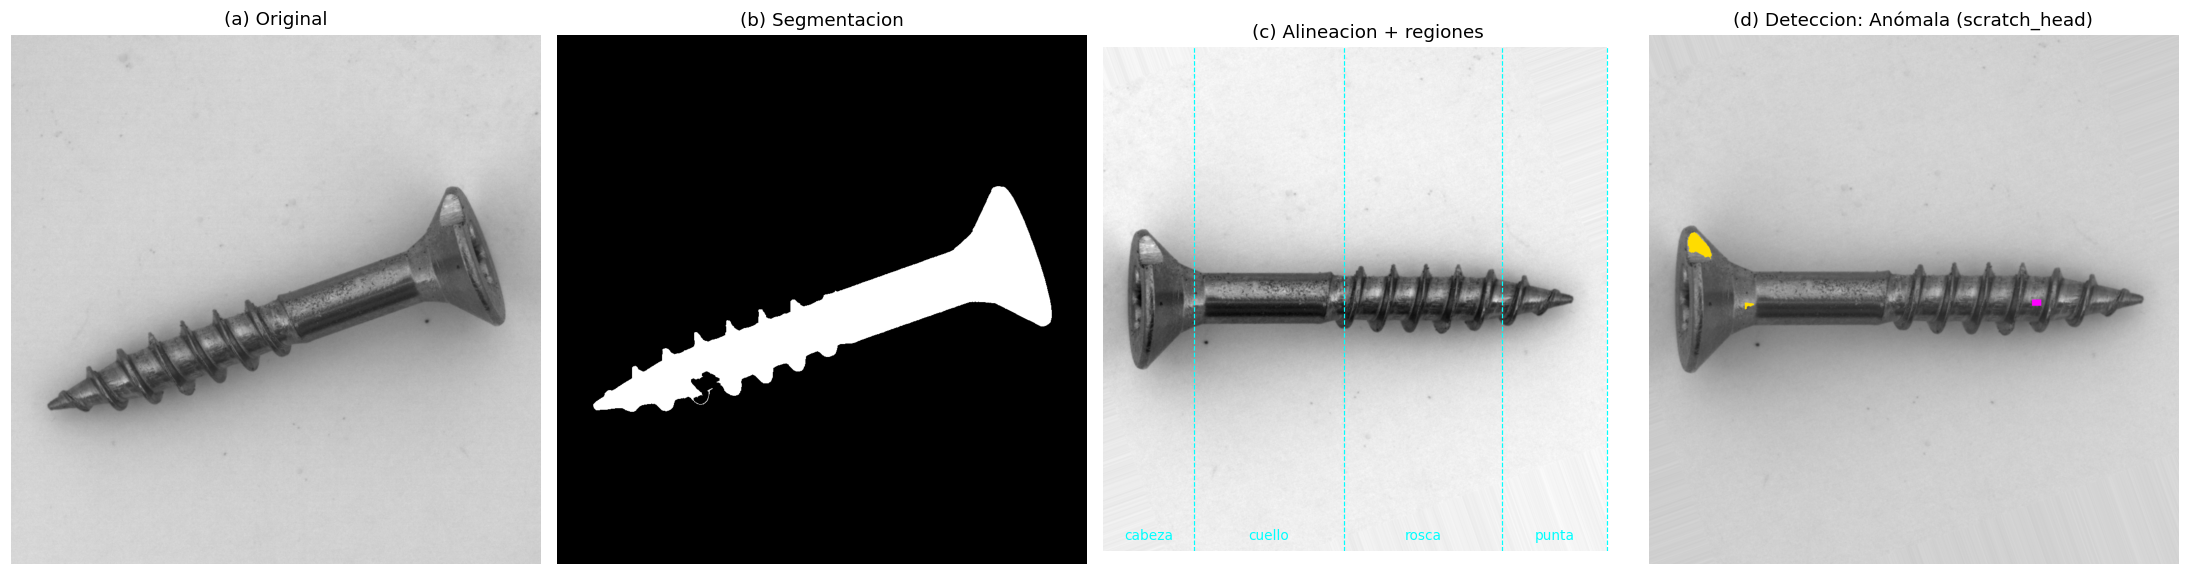
\includegraphics[width=\textwidth]{figuras/pipeline_etapas.png}
\caption{Etapas del pipeline sobre una imagen con arañazo en la cabeza:
(a) original, (b) máscara segmentada, (c) imagen alineada con las cuatro
regiones, (d) defecto detectado y diagnóstico.}
\label{fig:pipeline}
\end{figure}

\subsection{Fase 1: Preprocesamiento y segmentación}

El objetivo es aislar el tornillo del fondo mediante una máscara binaria.
El umbralado global de Otsu~\cite{otsu1979} resultó inadecuado: la sombra
difusa adyacente a la pieza posee niveles de gris cercanos al umbral y se
incluye erróneamente como objeto, inflando el área de la máscara hasta un
70\%. Se optó por una \textbf{segmentación basada en bordes}, fundamentada en
que la transición metal--fondo es un borde abrupto (gradiente fuerte) mientras
que la sombra es un degradé suave (gradiente débil). El procedimiento aplica un
suavizado gaussiano leve, el detector de Canny~\cite{canny1986} con umbrales
de histéresis $(40, 90)$, una dilatación que cierra el contorno, el relleno de
la componente de mayor área y una erosión simétrica que restaura el tamaño.
Con esta estrategia el área de las piezas sanas resulta prácticamente
constante ($\pm 1\%$), condición necesaria para la comparación posterior.

\subsection{Fase 2: Alineación espacial}

Para que la comparación píxel a píxel sea válida, todas las piezas deben
llevarse a una pose canónica. La orientación del eje longitudinal se obtiene
a partir de los momentos centrales de segundo orden de la máscara, que
proporcionan el ángulo del eje principal de inercia (equivalente a un análisis
de componentes principales):
\begin{equation}
\theta = \tfrac{1}{2}\arctan\!\left(\frac{2\,\mu_{11}}{\mu_{20}-\mu_{02}}\right).
\end{equation}
La pieza se rota a la horizontal y se determina la orientación cabeza-izquierda
comparando la masa de ambas mitades (la cabeza, más ancha, concentra más
píxeles). Finalmente, una única transformación afín combina rotación y
traslación para anclar el extremo de la cabeza en una columna fija y el eje
sobre la fila central. El anclaje se realiza \emph{por la cabeza} —estable en
todas las categorías— y no por el centroide, que se desplazaría ante un defecto
de punta y desalinearía toda la pieza. Una ambigüedad residual de espejo
vertical se resuelve por máxima superposición con la plantilla.

\subsection{Plantilla estadística (modelo de referencia)}

Las 41 máscaras alineadas se promedian píxel a píxel, obteniendo la fracción
de piezas sanas con metal en cada punto (Fig.~\ref{fig:plantilla}). De allí se
derivan dos zonas de decisión: el \textbf{núcleo} (metal en $\geq 97\%$ de los
sanos) y el \textbf{exterior} (metal en $\leq 3\%$). La franja intermedia
constituye una \emph{banda de tolerancia} que absorbe la variación natural de
la fase de la rosca. Adicionalmente se calculan la media y la desviación
estándar de la intensidad en cada píxel —base del detector de intensidad— y las
bandas de las envolventes de la rosca.

\begin{figure}[h]
\centering
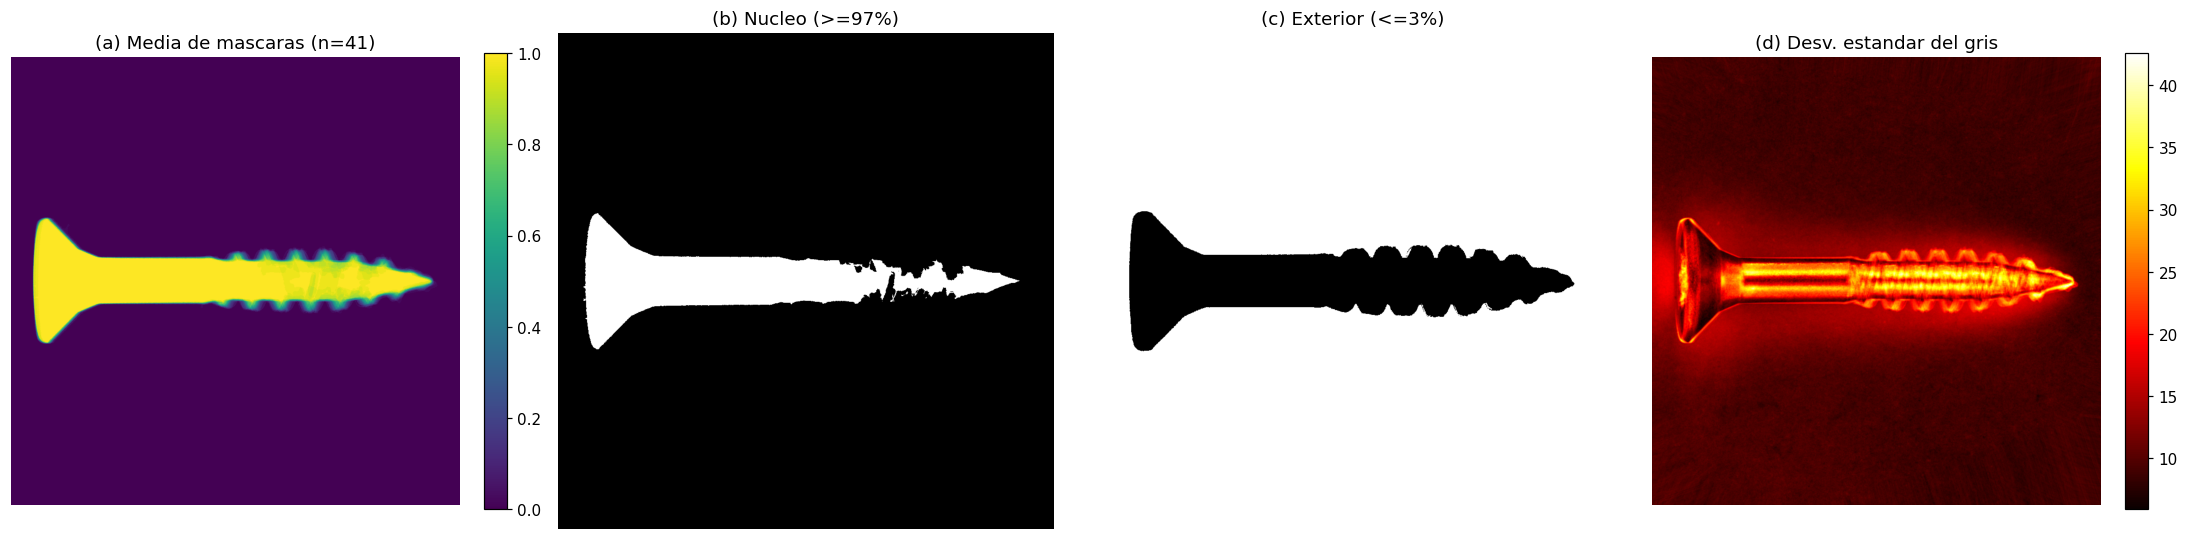
\includegraphics[width=\textwidth]{figuras/plantilla.png}
\caption{Plantilla estadística construida con las 41 piezas sanas:
(a) media de las máscaras, (b) zona núcleo, (c) zona exterior,
(d) desviación estándar de la intensidad (zonas claras = mayor variabilidad
natural, automáticamente toleradas).}
\label{fig:plantilla}
\end{figure}

\subsection{Fases 3--4: Detectores complementarios}

Sobre la imagen alineada se aplican tres detectores, cada uno dirigido a una
familia de defectos:

\paragraph{Detector de forma.} Compara la silueta contra las zonas
estadísticas mediante operaciones de conjuntos: el material \emph{faltante}
($\text{núcleo}\,\wedge\,\overline{\text{pieza}}$) revela roscas aplastadas y
puntas truncadas, y el material \emph{sobrante}
($\text{pieza}\,\wedge\,\text{exterior}$) revela rebabas y puntas dobladas.

\paragraph{Detector de intensidad.} Para cada píxel interior calcula el puntaje
estandarizado
\begin{equation}
z(x,y) = \frac{g(x,y) - \mu_{\text{good}}(x,y)}{\sigma_{\text{good}}(x,y) + \varepsilon},
\end{equation}
marcando como anómalos los píxeles que superan simultáneamente un criterio
estadístico ($|z|>2{,}5$) y uno visual ($|\Delta g|>20$ niveles). La tolerancia
se adapta espacialmente: donde los sanos varían mucho ($\sigma$ alta) el
detector es permisivo. Una corrección de iluminación por fila en el cuello,
basada en restar la mediana de cada fila, elimina los reflejos especulares que
se desplazan con la rotación axial del tornillo sin afectar los defectos
locales.

\paragraph{Detector de perfil de rosca.} Los defectos pequeños de las crestas
caen dentro de la banda de tolerancia del detector de forma. Para recuperarlos
se miden las \emph{envolventes} de la silueta (distancia del eje a crestas y
valles) mediante filtros de máximo y mínimo deslizante de un paso de rosca,
implementados como dilatación y erosión unidimensionales. Estas envolventes son
invariantes a la fase del filete y se comparan contra bandas estrechas
$[\min,\max]$ de las piezas sanas; toda excursión fuera de banda indica una
cresta dañada (Fig.~\ref{fig:perfil}).

\begin{figure}[h]
\centering
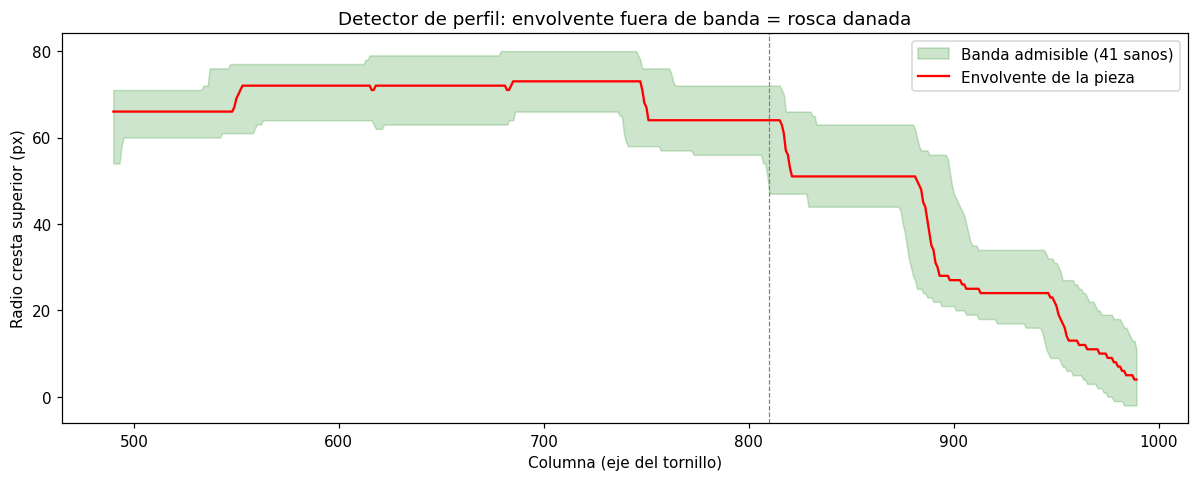
\includegraphics[width=0.85\textwidth]{figuras/perfil_rosca.png}
\caption{Detector de perfil: la envolvente de crestas de una pieza con rosca
dañada (rojo) escapa de la banda admisible de los tornillos sanos (verde) en
la zona del defecto.}
\label{fig:perfil}
\end{figure}

Cada detección se refina con apertura/cierre morfológico y filtrado por área de
componentes conexas, eliminando ruido puntual y detecciones espurias.

\subsection{Fase 5: Cuantificación y clasificación}

Las máscaras de defecto se resumen en un vector de diez \emph{scores}: dos por
cada una de las cuatro regiones (cabeza, cuello, rosca, punta) más dos del
perfil de rosca, normalizados por el área de la región. Cada score se contrasta
con un umbral calibrado con las piezas sanas según la regla
\begin{equation}
\text{umbral} = \max\big(\mu + 3\sigma,\; 1{,}25\cdot\text{máx}_{\text{sano}},\; \text{piso}\big),
\end{equation}
donde el término $\mu+3\sigma$ garantiza una tasa de falsos positivos cercana al
$0{,}13\%$ bajo hipótesis gaussiana. El \emph{nivel de anomalía} global es el
mayor cociente score/umbral: si supera la unidad, la pieza se clasifica como
anómala. El \textbf{tipo} de defecto se deduce de la región del score más
excedido (cabeza$\to$scratch\_head, cuello$\to$scratch\_neck,
rosca$\to$thread, punta$\to$manipulated\_front), produciendo un clasificador
completamente interpretable.

%==========================================================
\section{Resultados y Discusión}

El sistema se evaluó sobre las 160 imágenes del dataset, agrupando
\emph{thread\_side} y \emph{thread\_top} bajo la etiqueta común \emph{thread}.
La Tabla~\ref{tab:binario} resume la detección binaria (normal/anómala) por
categoría.

\begin{table}[h]
\centering
\caption{Exactitud de la detección binaria (normal vs.\ anómala) por categoría.}
\label{tab:binario}
\begin{tabular}{lcc}
\toprule
\textbf{Categoría} & \textbf{Detección} & \textbf{Exactitud} \\
\midrule
good (sanos)        & 41/41 & 100{,}0\% \\
scratch\_head       & 24/24 & 100{,}0\% \\
scratch\_neck       & 21/25 & 84{,}0\% \\
thread\_side        & 21/23 & 91{,}3\% \\
thread\_top         & 22/23 & 95{,}7\% \\
manipulated\_front  & 24/24 & 100{,}0\% \\
\midrule
\textbf{Global}     & \textbf{153/160} & \textbf{95{,}6\%} \\
\bottomrule
\end{tabular}
\end{table}

Considerando la detección de anomalías como problema binario, el sistema
alcanza una \emph{precisión} del 100\% (ningún tornillo sano fue rechazado),
una \emph{sensibilidad} (recall) del 94{,}1\% y un \emph{F1-score} de 0{,}97
(Tabla~\ref{tab:metricas}). La ausencia total de falsos positivos es un
resultado destacable en control de calidad, donde rechazar piezas correctas
tiene un costo directo. Los siete errores corresponden a falsos negativos:
defectos en el límite de detectabilidad (estrías de apenas $+10$ niveles de
gris o muescas menores a 10 px) que no pueden marcarse sin reducir los umbrales
al punto de comprometer la especificidad.

\begin{table}[h]
\centering
\caption{Métricas globales de la detección de anomalías (160 imágenes).}
\label{tab:metricas}
\begin{tabular}{lcccc}
\toprule
\textbf{Exactitud} & \textbf{Precisión} & \textbf{Recall} & \textbf{F1-Score} & \textbf{Falsos pos.} \\
\midrule
0{,}956 & 1{,}000 & 0{,}941 & 0{,}970 & 0 \\
\bottomrule
\end{tabular}
\end{table}

La Fig.~\ref{fig:detecciones} muestra ejemplos de inspección sobre una imagen
de cada categoría, con las evidencias de cada detector superpuestas en color.
Se observa que el detector de intensidad localiza con precisión los arañazos de
cabeza y cuello, mientras que los detectores de forma y perfil marcan las
deformaciones de rosca y punta.

\begin{figure}[h]
\centering
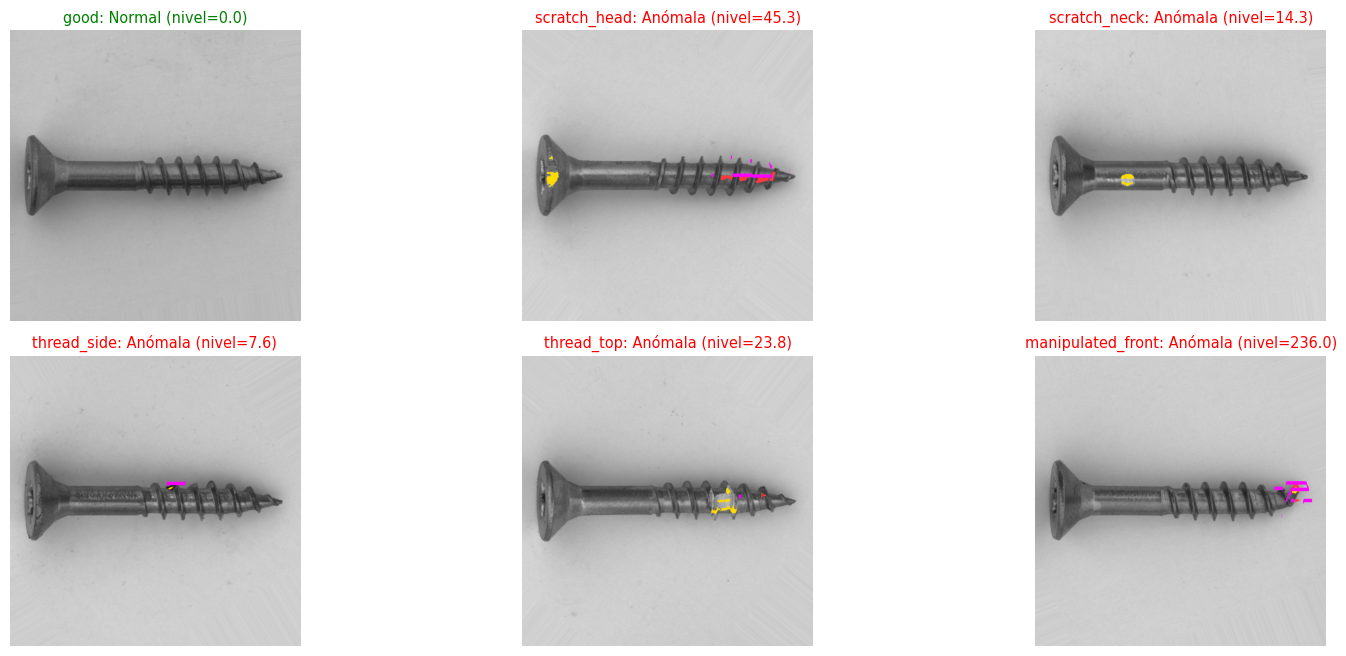
\includegraphics[width=\textwidth]{figuras/detecciones.png}
\caption{Resultados de inspección sobre una muestra de cada categoría. Las
evidencias se superponen por detector: forma (rojo), intensidad (amarillo) y
perfil de rosca (magenta). El tornillo sano (arriba-izquierda) no presenta
detecciones.}
\label{fig:detecciones}
\end{figure}

Respecto de la identificación del \emph{tipo} de defecto, la
Tabla~\ref{tab:confusion} presenta la matriz de confusión. La diagonal
concentra la mayoría de los casos; las confusiones más frecuentes se dan entre
\emph{scratch\_neck} y \emph{thread}, debido a que algunos raspones de cuello
se extienden hacia la zona de rosca, y a que la frontera entre ambas regiones
es difusa cuando el defecto se ubica en la transición.

\begin{table}[h]
\centering
\caption{Matriz de confusión del tipo de defecto (filas: real, columnas:
predicho). Etiquetas: g=good, sh=scratch\_head, sn=scratch\_neck, th=thread,
mf=manipulated\_front.}
\label{tab:confusion}
\small
\begin{tabular}{lccccc}
\toprule
 & \textbf{g} & \textbf{sh} & \textbf{sn} & \textbf{th} & \textbf{mf} \\
\midrule
good (g)               & 41 & 0  & 0  & 0  & 0  \\
scratch\_head (sh)     & 0  & 20 & 0  & 1  & 3  \\
scratch\_neck (sn)     & 4  & 0  & 12 & 5  & 4  \\
thread (th)            & 3  & 1  & 0  & 37 & 5  \\
manipulated\_front (mf)& 0  & 0  & 0  & 1  & 23 \\
\bottomrule
\end{tabular}
\end{table}

En conjunto, los resultados confirman que la combinación de detectores
complementarios sobre una etapa de normalización robusta permite alcanzar, con
técnicas exclusivamente clásicas, una exactitud competitiva en una de las
categorías más difíciles de MVTec AD, manteniendo plena interpretabilidad: para
cada pieza rechazada el sistema indica la región, el tipo y la severidad
(nivel de anomalía) del defecto.

%==========================================================
\section{Conclusiones}

Se desarrolló un sistema de inspección visual automática de tornillos basado
íntegramente en procesamiento digital de imágenes clásico, capaz de clasificar
piezas como normales o anómalas, identificar el tipo de defecto y localizarlo
sobre la imagen. La estrategia de detección por modelo de referencia, sustentada
en una normalización de pose precisa y en una plantilla estadística de la pieza
sana, demostró ser eficaz: el sistema alcanzó un 95{,}6\% de exactitud global
con cero falsos positivos sobre las 160 imágenes del dataset.

El aporte metodológico central fue el diseño de tres detectores complementarios
—forma, intensidad y perfil de rosca— derivados de un análisis previo del
dataset, donde cada uno resuelve las limitaciones de los otros: el detector de
intensidad con adaptación estadística local captura los arañazos sin confundir
los reflejos del metal, mientras que el detector de perfil mediante envolventes
invariantes a la fase recupera los defectos de rosca que escapan al análisis de
silueta. La calibración estadística de los umbrales con la regla de las tres
sigmas garantizó una especificidad perfecta.

Como líneas de trabajo futuro se identifican el refinamiento de la frontera
entre las regiones de cuello y rosca para reducir las confusiones de tipo, y la
incorporación de un análisis de textura local (por ejemplo, energía de
gradiente) que permita recuperar los arañazos de muy bajo contraste que
actualmente quedan por debajo del umbral de detección.

%==========================================================
\bibliographystyle{unsrtnat}
\bibliography{refs}

\end{document}
